\ifnum\solutions=1 {
  \clearpage
} \fi
\item\subquestionpoints{5}
\textbf{[Coding Problem] Classical (Unsupervised) EM Implementation.}
For this sub-question, we are only going to consider the $m$ unlabelled examples. Follow the instructions in \texttt{src/p03\_gmm.py} to implement the traditional EM algorithm, and run it on the unlabelled data-set until convergence.

Run three trials and use the provided plotting function to construct a scatter plot of the resulting assignments to clusters (one plot for each trial). Your plot should indicate cluster assignments with colors they got assigned to (\emph{i.e.,} the cluster which had the highest probability in the final E-step). 

\textbf{Note:} You only need to submit the three plots in your write-up. Your code will not be autograded.

\ifnum\solutions=1 {
  \begin{answer}

    Please see Figure \ref{fig:cluster}

\begin{figure}[htbp]
    \centering 
    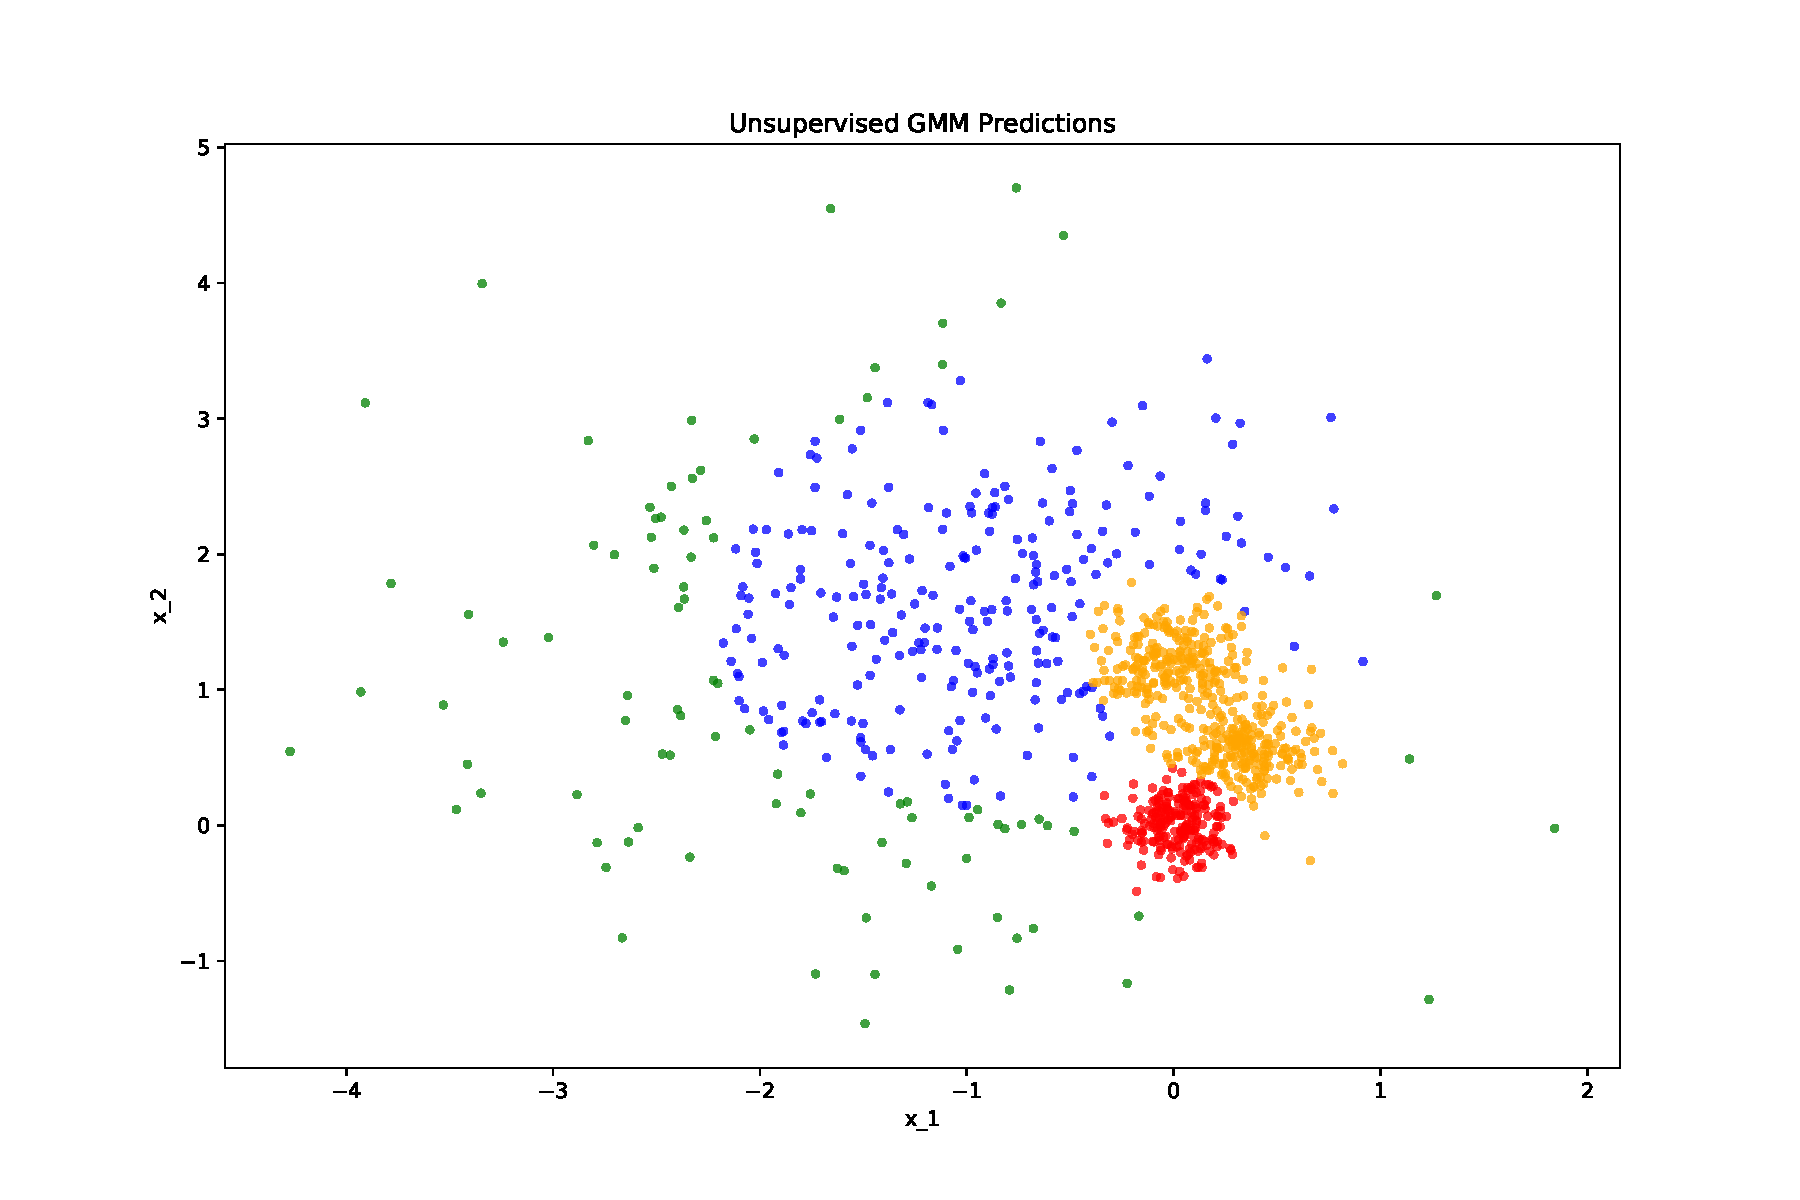
\includegraphics[width=0.7\linewidth]{pics/p03_pred_0.pdf}
    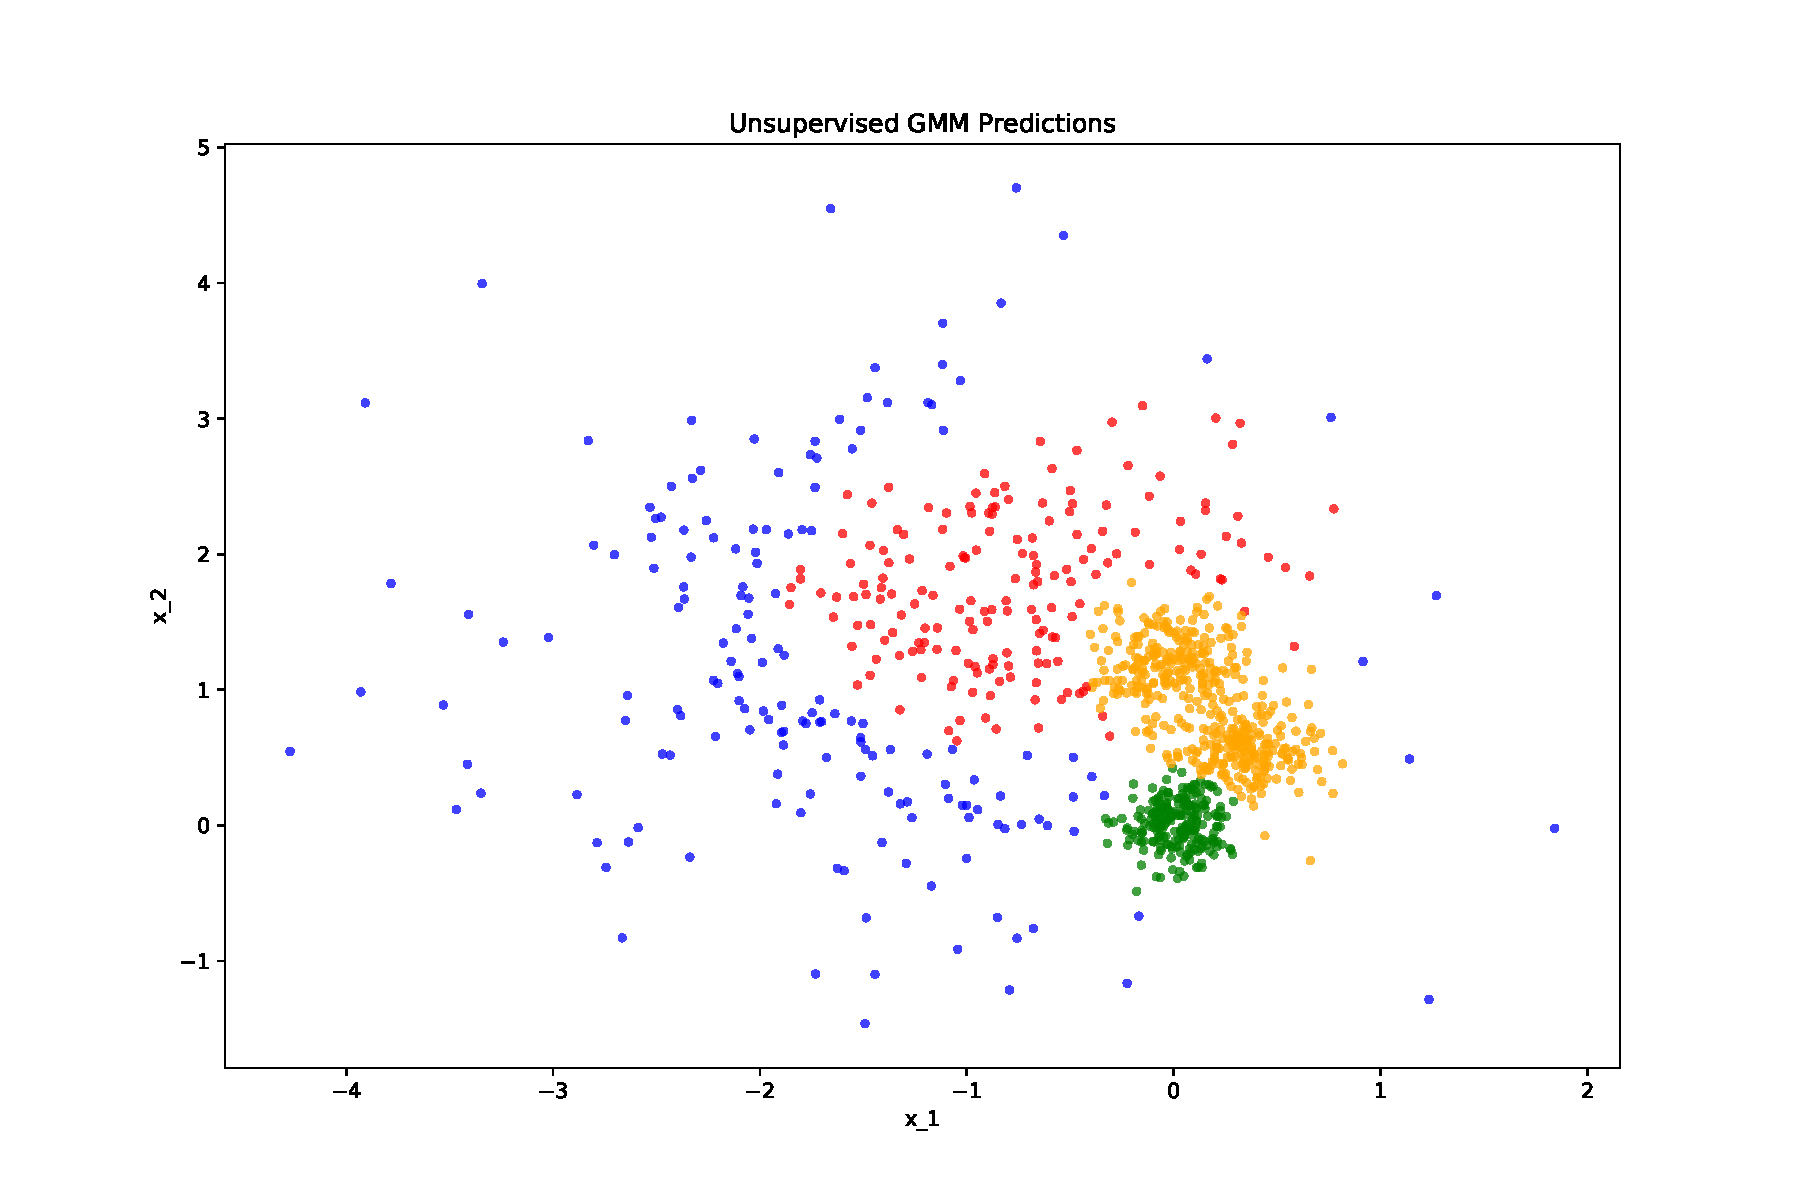
\includegraphics[width=0.7\linewidth]{pics/p03_pred_1.pdf}
    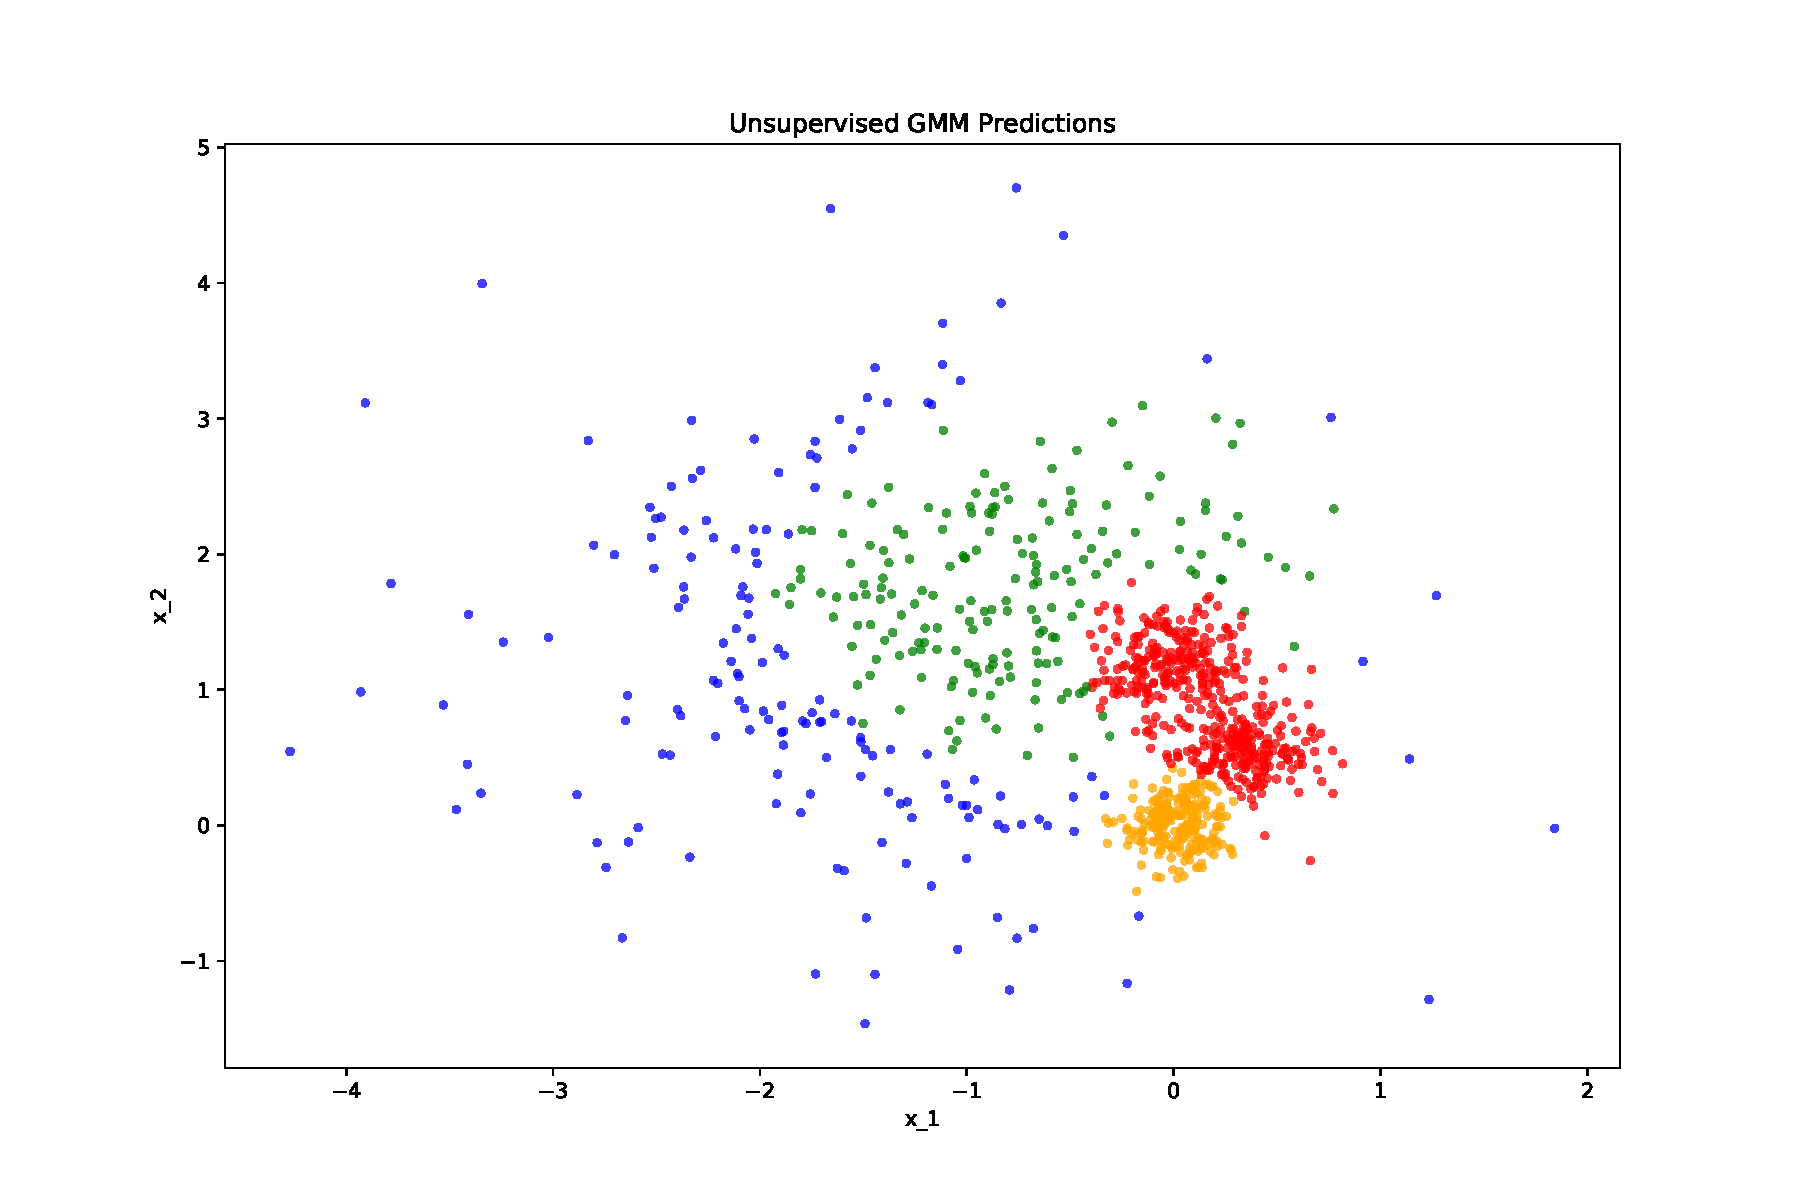
\includegraphics[width=0.7\linewidth]{pics/p03_pred_2.pdf}
    \caption{Clusters}
    \label{fig:cluster}
\end{figure}

\end{answer}

} \fi
